% EDC_Neutron_Junction_Model.tex
% Companion N to Paper 3: Neutron as Excited 5D Junction
% Version 0.1 (Draft) — 2026-01-20
% Build: XeLaTeX (Unicode)

\documentclass[11pt,a4paper]{article}

% ============================================================
%  PACKAGES
% ============================================================
\usepackage{fontspec}
\usepackage{amsmath,amssymb,amsthm}
\usepackage{mathtools}
\usepackage{physics}
\usepackage{geometry}

% FONTS (TeX Gyre Termes = Times-like with full OpenType support)
\IfFontExistsTF{TeX Gyre Termes}{%
  \setmainfont{TeX Gyre Termes}
  \setsansfont{TeX Gyre Heros}
}{%
  \setmainfont{Times New Roman}[Ligatures=TeX]
  \setsansfont{Helvetica}
}
\geometry{margin=2.5cm}
\usepackage{hyperref}
\hypersetup{
    colorlinks=true,
    linkcolor=blue,
    citecolor=blue,
    urlcolor=blue,
    pdfborder={0 0 0}
}
\usepackage{enumitem}
\usepackage{booktabs}
\usepackage{array}
\usepackage{xcolor}
\usepackage{tcolorbox}
\usepackage{tikz}
\usetikzlibrary{calc,angles,quotes,decorations.markings,decorations.pathmorphing}
\usepackage{gensymb}

% ============================================================
%  EPISTEMIC TAG COMMANDS
% ============================================================
\definecolor{tagDer}{RGB}{0,128,0}      % Green - Derived
\definecolor{tagDc}{RGB}{0,0,200}       % Blue - Deduced/Constrained
\definecolor{tagCal}{RGB}{200,0,0}      % Red - Calibrated
\definecolor{tagP}{RGB}{128,0,128}      % Purple - Postulated
\definecolor{tagBL}{RGB}{128,128,128}   % Gray - Baseline
\definecolor{tagI}{RGB}{255,140,0}      % Orange - Identified
\definecolor{tagOpen}{RGB}{200,100,0}   % Dark orange - Open

\newcommand{\tagDer}{\textcolor{tagDer}{\textbf{[Der]}}}
\newcommand{\tagDc}{\textcolor{tagDc}{\textbf{[Dc]}}}
\newcommand{\tagCal}{\textcolor{tagCal}{\textbf{[Cal]}}}
\newcommand{\tagP}{\textcolor{tagP}{\textbf{[P]}}}
\newcommand{\tagBL}{\textcolor{tagBL}{\textbf{[BL]}}}
\newcommand{\tagI}{\textcolor{tagI}{\textbf{[I]}}}
\newcommand{\tagOpen}{\textcolor{tagOpen}{\textbf{[OPEN]}}}
\newcommand{\tagDef}{\textcolor{tagDc}{\textbf{[Def]}}}

% ============================================================
%  THEOREM ENVIRONMENTS
% ============================================================
\newtheorem{postulate}{Postulate}
\newtheorem{definition}{Definition}[section]
\newtheorem{theorem}{Theorem}[section]
\newtheorem{lemma}[theorem]{Lemma}
\newtheorem{corollary}[theorem]{Corollary}
\newtheorem{proposition}[theorem]{Proposition}
\newtheorem{remark}{Remark}[section]

% ============================================================
%  CUSTOM COMMANDS
% ============================================================
\newcommand{\re}{r_e}
\newcommand{\Ztwo}{\mathbb{Z}_2}
\newcommand{\Ztri}{\mathbb{Z}_3}
\newcommand{\Zthree}{\mathbb{Z}_3}
\newcommand{\Zsix}{\mathbb{Z}_6}
\newcommand{\Sthree}{S^3}
\newcommand{\Stwo}{S^2}
\newcommand{\Bthree}{B^3}
\newcommand{\Mfive}{\mathcal{M}_5}
\newcommand{\Bfour}{\mathcal{B}_4}
\newcommand{\tension}{\tau}  % string/flux-tube tension (E/L)

% ============================================================
%  TITLE
% ============================================================
\title{\textbf{Neutron as Excited 5D Junction}\\[0.3em]
\Large in Elastic Diffusive Cosmology\\[0.5em]
\normalsize (Companion N to Paper~3: NJSR Edition)\\[0.3em]
\footnotesize Draft v0.1 (January 2026)}
\author{Igor Gr\v{c}man}
\date{January 2026\\[0.5em]
\small DOI: \href{https://doi.org/10.5281/zenodo.18315110}{10.5281/zenodo.18315110}\\[0.3em]
\small Repository: \href{https://github.com/igorgrcman/elastic-diffusive-cosmology}{github.com/igorgrcman/elastic-diffusive-cosmology}\\[0.2em]
\footnotesize (Public artifacts for this paper are in the \texttt{edc\_papers} folder.)}

% ============================================================
%  DOCUMENT
% ============================================================
\begin{document}

\maketitle

% ------------------------------------------------------------
%  RELATED DOCUMENTS
% ------------------------------------------------------------
\begin{center}
\small\textbf{Related Documents:}\\[0.1cm]
\footnotesize
\emph{Neutron Lifetime from 5D Membrane Cosmology} (DOI: \href{https://doi.org/10.5281/zenodo.18262721}{10.5281/zenodo.18262721})\\[0.05cm]
\emph{Framework v2.0} (DOI: \href{https://doi.org/10.5281/zenodo.18299085}{10.5281/zenodo.18299085})\\[0.05cm]
\textbf{Companions:}\\
A: \emph{Effective Lagrangian} (\href{https://doi.org/10.5281/zenodo.18292841}{DOI}) ~$\cdot$~
B: \emph{WKB Prefactor} (\href{https://doi.org/10.5281/zenodo.18299637}{DOI})\\
C: \emph{5D Reduction} (\href{https://doi.org/10.5281/zenodo.18299751}{DOI}) ~$\cdot$~
D: \emph{Selection Rules} (\href{https://doi.org/10.5281/zenodo.18299855}{DOI})\\
E: \emph{Symmetry Ops} (\href{https://doi.org/10.5281/zenodo.18300199}{DOI}) ~$\cdot$~
F: \emph{Proton Junction} (\href{https://doi.org/10.5281/zenodo.18302953}{DOI})\\
G: \emph{Mass Difference} (\href{https://doi.org/10.5281/zenodo.18303494}{DOI}) ~$\cdot$~
H: \emph{Weak Interactions} (\href{https://doi.org/10.5281/zenodo.18307539}{DOI})\\[0.05cm]
\textbf{This:} N: \emph{Neutron Junction} (\href{https://doi.org/10.5281/zenodo.18315110}{DOI})
\end{center}

% ------------------------------------------------------------
%  ABSTRACT
% ------------------------------------------------------------
\begin{abstract}
We establish the neutron as an \textbf{excited 5D junction state} within Elastic Diffusive Cosmology (EDC). The neutron shares the same three-arm junction topology as the proton (Companion F), but is displaced from the local Steiner minimum---the universal $120\degree$ optimum in the tangent metric. This excitation couples to the bulk-facing side of a thick brane, pumping energy into brane-layer modes. The observer-side frozen projection boundary then organizes the released energy into allowed weak-channel outputs ($e^- + \bar{\nu}_e$).

\textbf{Calibration boundary:} The neutron lifetime $\tau_n \approx 879\,\text{s}$ is treated as a \textbf{baseline observable} \tagBL{}, not as a prediction of this companion. The lifetime value enters only as a phenomenological check; no parameters are fitted to it here.

\textbf{Epistemic status:} The junction postulate is \tagP{} (inherited from Companion F). Given this postulate, the neutron's excited nature is \tagP{}, while the Steiner relaxation mechanism is \tagDc{}. The thick-brane pumping and frozen projection remain \tagOpen{} at the microphysics level.
\end{abstract}

\tableofcontents

\vspace{1em}
\begin{tcolorbox}[colback=blue!5,colframe=blue!40!black,title=\textbf{Cornerstone: Neutron in EDC}]
In the EDC program, the neutron is modeled as an excited 5D junction state: the same three-arm junction core as the proton, but displaced from the local Steiner minimum (the universal $120\degree$ optimum in the tangent metric). This excitation couples to the bulk-facing side of a thick brane, pumping energy into brane-layer modes. The observer-side frozen projection boundary then organizes the released energy into allowed weak-channel outputs (e.g., $e^-$ and $\bar{\nu}_e$), while overall bulk--brane conservation remains anchored to Framework v2.0, Remark~4.5.

\medskip
\textbf{Epistemic status:}
\begin{itemize}[nosep]
    \item $120\degree$ as local optimum: \tagDer{}/\tagDc{} (geometric, from Companion F)
    \item Neutron = excited junction: \tagP{} (object assumption)
    \item Thick-brane pumping + frozen output mapping: \tagP{}/\tagOpen{}
\end{itemize}
\end{tcolorbox}

\newpage

% ============================================================
%  SECTION 1: MOTIVATION AND SCOPE
% ============================================================
\section{Motivation and Scope}
\label{sec:motivation}

\subsection{The Gap: Neutron Object Model}

Companion F establishes the proton as a Y-junction in 5D---a three-arm flux-tube network meeting at $120\degree$ angles (Steiner configuration). Companion G derives the neutron-proton mass difference from $\Zsix$ symmetry breaking. Companion H describes weak interactions as junction transitions mediated by thick-brane microphysics.

\textbf{What is missing:} A clear statement of \emph{what the neutron is} as a 5D object, analogous to Companion F's treatment of the proton.

\subsection{Purpose of This Companion}

This document provides the \textbf{neutron backbone}:
\begin{enumerate}
    \item Define the neutron as an excited 5D junction state \tagP{}
    \item Show that instability arises from displacement from Steiner minimum \tagDc{}
    \item Connect junction oscillation to thick-brane energy pumping \tagP{}/\tagOpen{}
    \item Describe the frozen projection boundary as organizing outputs \tagDc{}/\tagP{}
    \item Identify the bridge to the NJSR paper's WKB treatment \tagOpen{}
\end{enumerate}

\subsection{What This Companion Does NOT Do}

\begin{itemize}
    \item Does NOT derive the lifetime $\tau_n \approx 879\,\text{s}$ from first principles (remains \tagCal{} via the NJSR paper's WKB barrier)
    \item Does NOT derive the V--A structure of weak interactions (Standard Model input \tagBL{})
    \item Does NOT derive the thick-brane coupling constant (remains \tagOpen{})
\end{itemize}

\subsection{Epistemic Hierarchy}

\begin{center}
\begin{tabular}{lll}
\toprule
\textbf{Level} & \textbf{Content} & \textbf{Status} \\
\midrule
Inherited & Baryon = 3-arm junction in 5D bulk & \tagP{} (from F) \\
Inherited & Equal tensions $\Rightarrow$ $120\degree$ angles & \tagDer{} (from F) \\
Postulate & Neutron = excited (non-Steiner) junction & \tagP{} \\
Definition & Collective coordinate $q = |\hat{e}_1 + \hat{e}_2 + \hat{e}_3|/3$ & \tagDef{} \\
Consequence & Excitation carries geometric energy & \tagDc{} \\
Model & Ring mode + 3 springs (heuristic) & \tagI{}/\tagP{} \\
Open & Thick-brane pumping mechanism & \tagOpen{} \\
Open & WKB--damping bridge & \tagOpen{} \\
\bottomrule
\end{tabular}
\end{center}

% ============================================================
%  SECTION 2: THICK-BRANE SETTING
% ============================================================
\section{Thick-Brane Microphysics}
\label{sec:thick-brane}

This section establishes the foundational thick-brane microphysical picture for interpreting neutron decay. The goal is to provide a clear physical bridge: how bulk dynamics (junction transitions) produce observed 3D particles (electrons, neutrinos) through the mediation of a thick brane with finite extent.

\textbf{Note:} This section reproduces key definitions from Companion H (DOI: \href{https://doi.org/10.5281/zenodo.18307539}{10.5281/zenodo.18307539}) to make Companion N self-contained. Companion H remains the canonical source for the full thick-brane formalism.

% -----------------------------------------------------------------------------
\subsection{Thin Brane vs Thick Brane: Why Thickness Matters}
\label{subsec:thin_vs_thick}
% -----------------------------------------------------------------------------

\begin{definition}[Thin Brane vs Thick Brane \textup{\tagDef}]
\label{def:thin_thick_brane}
\begin{itemize}
    \item \textbf{Thin brane:} A mathematical idealization where the 4D world-volume has zero thickness in the extra dimension ($\delta \to 0$). Fields are strictly confined to a hypersurface. Computationally convenient but obscures the physical interface structure.

    \item \textbf{Thick brane:} A regularized model where the brane has finite thickness $\delta > 0$ in the extra dimension. The brane possesses two distinct faces:
    \begin{enumerate}
        \item \textbf{Bulk-facing side} ($y = -\delta/2$): The interface where bulk fields couple to brane dynamics
        \item \textbf{Observer-facing side} ($y = +\delta/2$): The interface where effective 3D/4D physics emerges
    \end{enumerate}
\end{itemize}
\end{definition}

\noindent\textbf{Why thick brane for weak processes?} The thick-brane picture provides:
\begin{enumerate}
    \item \textbf{Regularization:} Avoids singular delta-function sources in the 5D equations
    \item \textbf{Two-face structure:} Distinguishes where energy enters (bulk-facing) from where particles emerge (observer-facing)
    \item \textbf{Localization mechanism:} Brane-layer modes have finite transverse extent, enabling mode selection
    \item \textbf{Frozen boundary interpretation:} The one-way valve becomes a property of the observer-facing interface
\end{enumerate}

% -----------------------------------------------------------------------------
\subsection{Core Definitions: Bulk-Core, Brane-Layer, 3D Outputs}
\label{subsec:core_definitions}
% -----------------------------------------------------------------------------

\begin{definition}[Bulk-Core \textup{\tagP}]
\label{def:bulk_core}
The \textbf{bulk-core} comprises the degrees of freedom of the Y-junction and its three attached flux-tube arms, located in the 5D bulk away from the brane. The collective coordinate $q(t)$ parametrizes the junction configuration:
\begin{itemize}
    \item $q = 0$: proton configuration (ground state $\ket{0}$, Steiner minimum)
    \item $q > 0$: neutron configuration (excited state $\ket{1}$, displaced from Steiner)
\end{itemize}
Bulk-core dynamics are governed by the effective potential $V(q)$ and effective mass $M_{\mathrm{eff}}(q)$.
\end{definition}

\begin{definition}[Brane-Layer Modes \textup{\tagP}]
\label{def:brane_layer}
The \textbf{brane-layer} is the region of finite thickness $\delta$ where the 4D membrane resides. Within this layer, localized field excitations $\phi(y, t)$ propagate, where $y \in [-\delta/2, +\delta/2]$ denotes coordinates across the brane thickness. These are phonon-like or soliton-like modes of the membrane:
\begin{itemize}
    \item \textbf{Localized deformations:} electrons, positrons (topological winding)
    \item \textbf{Delocalized waves:} neutrinos, antineutrinos (lepton-number carriers)
\end{itemize}
\end{definition}

\begin{definition}[Observed 3D Particle States \textup{\tagDef}]
\label{def:3d_outputs}
\textbf{Observed 3D particle states} are the effective outputs that emerge on the observer-facing side of the brane. These are what laboratory detectors register. The relation to brane-layer modes:
\[
\text{Brane-layer mode } \phi(y,t) \xrightarrow{\mathcal{P}_{\mathrm{frozen}}} \text{3D particle state}
\]
This projection is mediated by the frozen projection operator (Def.~\ref{def:frozen_operator}).
\end{definition}

% -----------------------------------------------------------------------------
\subsection{The Thick-Brane Geometry}
\label{subsec:thick_brane_geometry}
% -----------------------------------------------------------------------------

\begin{figure}[h]
\centering
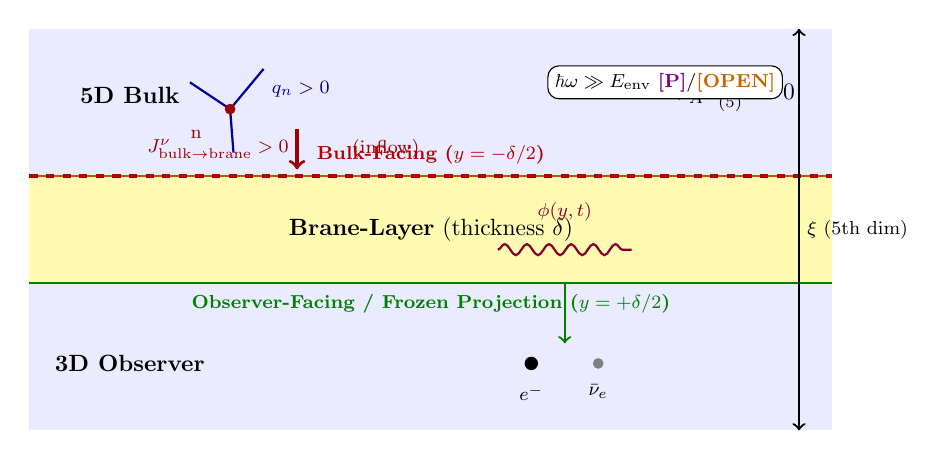
\begin{tikzpicture}[scale=0.85, transform shape]
    % Bulk region (5D)
    \fill[blue!8] (-6,-3) rectangle (6,3);

    % Brane layer (thick)
    \fill[yellow!30] (-6,-0.8) rectangle (6,0.8);
    \draw[thick, orange!70!black] (-6,0.8) -- (6,0.8);
    \draw[thick, orange!70!black] (-6,-0.8) -- (6,-0.8);

    % Bulk-facing side
    \draw[very thick, red!70!black, dashed] (-6,0.8) -- (6,0.8);
    \node[red!70!black, above] at (0,0.85) {\footnotesize\textbf{Bulk-Facing ($y = -\delta/2$)}};

    % Observer-facing side (frozen projection)
    \draw[thick, green!50!black] (-6,-0.8) -- (6,-0.8);
    \node[green!50!black, below] at (0,-0.85) {\footnotesize\textbf{Observer-Facing / Frozen Projection ($y = +\delta/2$)}};

    % Labels for regions
    \node at (-4.5,2) {\textbf{5D Bulk}};
    \node at (4.5,2) {$\nabla_A T^{AB}_{(5)} = 0$};
    \node at (0,0) {\textbf{Brane-Layer} (thickness $\delta$)};
    \node at (-4.5,-2) {\textbf{3D Observer}};

    % Y-junction in bulk (neutron excited state)
    \begin{scope}[shift={(-3,1.8)}]
        \draw[thick, blue!60!black] (0,0) -- (0.5,0.6);
        \draw[thick, blue!60!black] (0,0) -- (-0.6,0.4);
        \draw[thick, blue!60!black] (0,0) -- (0.05,-0.65);
        \fill[red!60!black] (0,0) circle (0.08);
        \node[blue!60!black, right] at (0.5,0.3) {\footnotesize $q_n > 0$};
        \node[red!60!black, below left, font=\footnotesize] at (-0.3,-0.2) {n};
    \end{scope}

    % Energy flow arrow (inflow)
    \draw[->, very thick, red!60!black] (-2,1.5) -- (-2,0.9);
    \node[red!60!black, left] at (-2,1.2) {\footnotesize $J^\nu_{\mathrm{bulk}\to\mathrm{brane}} > 0$};
    \node[red!60!black, right] at (-1.3,1.2) {\footnotesize (inflow)};

    % Brane-layer mode
    \draw[thick, purple!70!black, decorate, decoration={snake, amplitude=2pt, segment length=8pt}]
        (1,-0.3) -- (3,-0.3);
    \node[purple!70!black, above] at (2,0) {\footnotesize $\phi(y,t)$};

    % 3D outputs (electron + antineutrino)
    \fill[black] (1.5,-2) circle (0.1);
    \node[below] at (1.5,-2.2) {\footnotesize $e^-$};
    \fill[gray] (2.5,-2) circle (0.08);
    \node[below] at (2.5,-2.2) {\footnotesize $\bar{\nu}_e$};
    \draw[->, thick, green!50!black] (2,-0.8) -- (2,-1.7);

    % Dimension labels
    \draw[<->, thick] (5.5,-3) -- (5.5,3);
    \node[right] at (5.5,0) {\footnotesize $\xi$ (5th dim)};

    % Criterion box
    \node[draw, fill=white, rounded corners, inner sep=3pt] at (3.5,2.2)
        {\footnotesize $\hbar\omega \gg E_{\mathrm{env}}$ \tagP/\tagOpen};
\end{tikzpicture}
\caption{Thick-brane geometry for neutron decay. The neutron (Y-junction with $q_n > 0$, displaced from Steiner) relaxes in the 5D bulk, releasing energy as inflow ($J^\nu_{\mathrm{bulk}\to\mathrm{brane}} > 0$) through the bulk-facing boundary. This excites brane-layer modes $\phi(y,t)$, which propagate through the brane thickness and emerge as 3D particle outputs ($e^- + \bar{\nu}_e$) via the frozen projection at the observer-facing boundary.}
\label{fig:thick_brane_geometry}
\end{figure}

% -----------------------------------------------------------------------------
\subsection{The Brane as ``Glass Window''}

\begin{tcolorbox}[colback=yellow!5,colframe=orange!50!black,title=\textbf{Conceptual Picture \tagP}]
\begin{center}
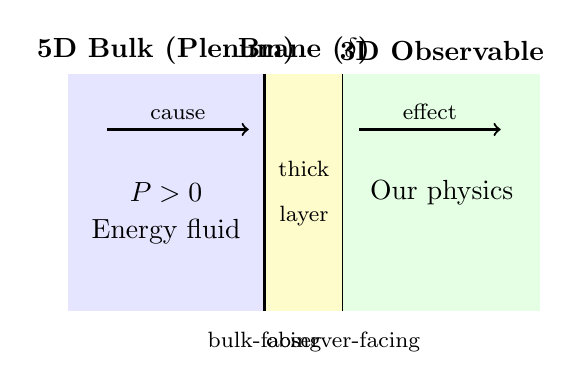
\begin{tikzpicture}[scale=1.0]
    % Bulk side
    \fill[blue!10] (-3,-1.5) rectangle (-0.5,1.5);
    \node at (-1.75,1.8) {\textbf{5D Bulk (Plenum)}};
    \node at (-1.75,0) {$P > 0$};
    \node at (-1.75,-0.5) {Energy fluid};

    % Brane
    \fill[yellow!20] (-0.5,-1.5) rectangle (0.5,1.5);
    \draw[very thick] (-0.5,-1.5) -- (-0.5,1.5);
    \draw[very thick] (0.5,-1.5) -- (0.5,1.5);
    \node at (0,1.8) {\textbf{Brane ($\delta$)}};
    \node[font=\footnotesize] at (0,0.3) {thick};
    \node[font=\footnotesize] at (0,-0.3) {layer};

    % Observer side
    \fill[green!10] (0.5,-1.5) rectangle (3,1.5);
    \node at (1.75,1.8) {\textbf{3D Observable}};
    \node at (1.75,0) {Our physics};

    % Labels
    \node[font=\footnotesize] at (-0.5,-1.9) {bulk-facing};
    \node[font=\footnotesize] at (0.5,-1.9) {observer-facing};

    % Arrows
    \draw[->,thick] (-2.5,0.8) -- (-0.7,0.8) node[midway,above,font=\footnotesize] {cause};
    \draw[->,thick] (0.7,0.8) -- (2.5,0.8) node[midway,above,font=\footnotesize] {effect};
\end{tikzpicture}
\end{center}

\textbf{Key idea:} The brane has TWO sets of boundary conditions:
\begin{itemize}[nosep]
    \item \textbf{Left (bulk-facing):} BC toward 5D bulk (Plenum, energy fluid)
    \item \textbf{Right (observer-facing):} BC toward 3D observable universe (our physics)
\end{itemize}
Physics in 5D is the \textbf{cause}; 3D observations are the \textbf{effect}.
\end{tcolorbox}

\subsection{Bulk--Brane Energy Exchange}
\label{subsec:energy_exchange}

\begin{tcolorbox}[colback=gray!5!white,colframe=gray!60!black,title={\small Framework v2.0, Remark 4.5 --- Canonical Energy Conservation}]
\textbf{(1) 5D closure:}
\begin{equation}
\nabla_A T^{AB}_{(5)} = 0 \quad (A,B = 0,\dots,4)
\end{equation}

\textbf{(2) Brane open subsystem:}
\begin{equation}
\nabla_\mu T^{\mu\nu}_{\mathrm{brane}} = -\,J^\nu_{\mathrm{bulk}\to\mathrm{brane}} \quad (\mu,\nu = 0,\dots,3)
\end{equation}

\textbf{Sign convention:} $J^\nu_{\mathrm{bulk}\to\mathrm{brane}} > 0$ denotes net \emph{inflow} into the brane sector.

\textbf{(3) Junction determination:} The exchange current $J^\nu_{\mathrm{bulk}\to\mathrm{brane}}$ is fixed by the chosen bulk--brane boundary/junction conditions (e.g., Israel-type matching).

\textbf{(4) Ledger language:} The ``conservation ledger'' is bookkeeping language for bulk--brane closure, not a new law.

\vspace{0.2cm}
\noindent\textit{\footnotesize This block is quoted verbatim from Framework v2.0, Remark 4.5; Framework remains the canonical source.}
\end{tcolorbox}

\begin{remark}[Brane Subsystem is Open \textup{\tagDef}]
\label{rem:brane-open}
The brane, viewed as a subsystem, can exchange energy-momentum with the bulk. The apparent ``nonconservation'' $\nabla_\mu T^{\mu\nu}_{\mathrm{brane}} \neq 0$ is not a violation of physics---it reflects that the brane is an open system. Conservation is restored when bulk and brane are combined:
\[
\Delta E_{\mathrm{brane}} + \Delta E_{\mathrm{bulk}} = 0
\]
\end{remark}

The thick-brane allows energy to flow from bulk structures (junctions) into brane-localized modes, which then appear as observable particles on the 3D side.

\subsection{Frozen Projection Boundary}

\begin{definition}[Frozen Projection \textup{\tagDc}/\textup{\tagP}]
\label{def:frozen-projection}
The \textbf{frozen projection boundary} is the observer-facing interface where:
\begin{enumerate}[nosep]
    \item High-frequency bulk modes are adiabatically eliminated (``frozen'')
    \item Only allowed channels (selection rules) can carry energy to 3D
    \item Acts as a \textbf{one-way valve}: INFLOW allowed, OUTFLOW suppressed
\end{enumerate}
\end{definition}

For neutron decay, this boundary organizes the released junction energy into the $\beta^-$ channel: $e^- + \bar{\nu}_e + \text{recoil}$.

% ============================================================
%  SECTION 3: NEUTRON AS EXCITED JUNCTION
% ============================================================
\section{Neutron as Excited Junction: Ontology}
\label{sec:ontology}

\subsection{Same Topology, Different State}

\begin{postulate}[Neutron as Excited Junction \textup{\tagP}]
\label{post:neutron-excited}
In 5D EDC, the neutron is a three-arm flux-tube junction with the \textbf{same topological structure} as the proton, but in an \textbf{excited state}---displaced from the Steiner minimum.
\end{postulate}

\begin{center}
\begin{tabular}{lcc}
\toprule
& \textbf{Proton} & \textbf{Neutron} \\
\midrule
Topology & Y-junction (3 arms) & Y-junction (3 arms) \\
Arm angles & $120\degree$ (Steiner) & $\neq 120\degree$ (excited) \\
Energy state & Ground state (minimum) & Metastable (excited) \\
Stability & Stable & Unstable ($\tau \approx 879$ s) \\
Charge (Q) & +1 & 0 \\
\bottomrule
\end{tabular}
\end{center}

\subsection{Collective Coordinate}

\begin{definition}[Collective Coordinate $q$ \textup{\tagDef}]
\label{def:collective-q}
Let $\hat{e}_i$ ($i = 1,2,3$) be the unit tangent vectors at the junction. The collective coordinate measuring departure from Steiner symmetry is:
\begin{equation}
\boxed{q \equiv \frac{1}{3}\left| \hat{e}_1 + \hat{e}_2 + \hat{e}_3 \right|}
\label{eq:q-def}
\end{equation}
\end{definition}

\begin{proposition}[Range and Interpretation \textup{\tagDer}]
\label{prop:q-range}
The collective coordinate satisfies:
\begin{itemize}
    \item $q = 0$: Steiner configuration ($\hat{e}_1 + \hat{e}_2 + \hat{e}_3 = 0$) $\Rightarrow$ \textbf{proton}
    \item $q = 1$: Maximal asymmetry (all arms parallel) $\Rightarrow$ unphysical limit
    \item $0 < q < 1$: Excited states, including \textbf{neutron}
\end{itemize}
\end{proposition}

\begin{proof}
For unit vectors summing to zero (Steiner), $|\sum \hat{e}_i| = 0$, hence $q = 0$. For all parallel, $|\sum \hat{e}_i| = 3$, hence $q = 1$. Intermediate configurations give $0 < q < 1$.
\end{proof}

\begin{remark}[Neutron value of $q$ \textup{\tagI}/\textup{\tagOpen}]
\label{rem:q-neutron}
Based on $\Zsix$ symmetry arguments (Companion G), the neutron corresponds to approximately:
\begin{equation}
q_n \approx \frac{1}{3} \quad \text{(or equivalently, half-Steiner displacement)}
\end{equation}
The precise value and its derivation from first principles remain \tagOpen{}. Current estimates give $q_n \approx 0.31$ from phenomenological matching.
\end{remark}

\subsection{Energy from Displacement}

\begin{lemma}[Geometric Excitation Energy \textup{\tagDc}]
\label{lem:excitation-energy}
Any displacement from the Steiner minimum ($q = 0$) carries positive geometric energy:
\begin{equation}
E_{\text{geom}}(q) = E_0 + \kappa_q \, q^2 + O(q^4)
\label{eq:energy-taylor}
\end{equation}
where $\kappa_q > 0$ is the stiffness of the junction against asymmetric deformations.
\end{lemma}

\begin{proof}
The Steiner point is a local minimum of the total weighted length (Companion F, Theorem 4.1). Near a minimum, the energy expands as a positive-definite quadratic form to leading order.
\end{proof}

\begin{corollary}[Instability \textup{\tagDc}]
The neutron ($q_n > 0$) has higher energy than the proton ($q = 0$). This energy difference drives relaxation toward the Steiner minimum.
\end{corollary}

\begin{figure}[h]
\centering
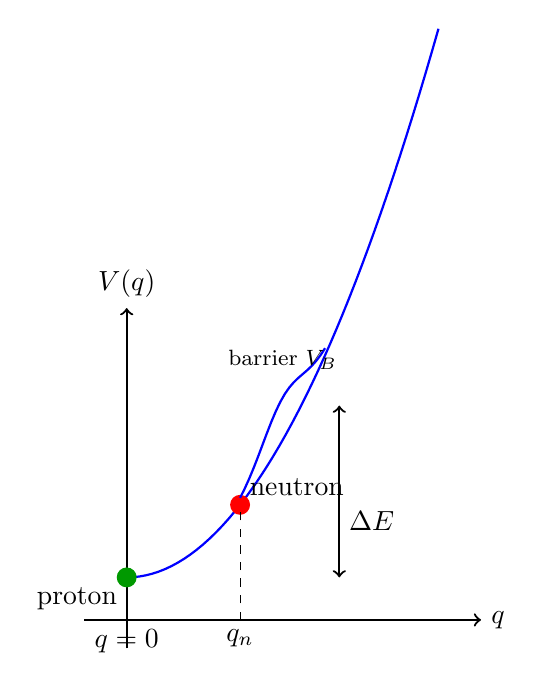
\begin{tikzpicture}[scale=1.8]
    % Potential well
    \draw[thick,->] (-0.3,0) -- (2.5,0) node[right] {$q$};
    \draw[thick,->] (0,-0.2) -- (0,2.2) node[above] {$V(q)$};

    % Potential curve
    \draw[thick,blue,domain=0:2.2,samples=50] plot (\x, {0.3 + 0.8*\x*\x});

    % Proton minimum
    \fill[green!60!black] (0,0.3) circle (2pt);
    \node[below left] at (0,0.3) {proton};
    \node[below] at (0,0) {$q=0$};

    % Neutron excited
    \fill[red] (0.8,0.812) circle (2pt);
    \node[above right] at (0.8,0.812) {neutron};
    \draw[dashed] (0.8,0) -- (0.8,0.812);
    \node[below] at (0.8,0) {$q_n$};

    % Energy difference
    \draw[<->,thick] (1.5,0.3) -- (1.5,0.812+0.7);
    \node[right] at (1.5,0.7) {$\Delta E$};

    % Barrier (schematic)
    \draw[thick,blue,domain=0.8:1.4,samples=20] plot (\x, {0.3 + 0.8*\x*\x + 0.3*exp(-20*(\x-1.1)*(\x-1.1))});
    \node[above,font=\footnotesize] at (1.1,1.7) {barrier $V_B$};
\end{tikzpicture}
\caption{Schematic potential $V(q)$ for the junction coordinate. The proton sits at $q=0$ (Steiner minimum); the neutron at $q_n > 0$ (metastable excited state). A barrier $V_B$ separates neutron from proton, determining the tunneling lifetime.}
\label{fig:potential}
\end{figure}

% ============================================================
%  SECTION 4: MECHANICS PICTURE
% ============================================================
\section{Mechanics Picture: Ring + 3 Springs}
\label{sec:mechanics}

\subsection{Heuristic Model}

To build intuition for the junction dynamics, we introduce a mechanical analogy.

\begin{tcolorbox}[colback=green!5,colframe=green!40!black,title=\textbf{Mechanical Analogy \tagI/\tagP}]
\textbf{Ring + 3 Springs Model:}

Consider a circular ring of radius $R$ with three springs attached at angles $\theta_1, \theta_2, \theta_3$, each pulling toward the center with spring constant $k$. The springs represent flux-tube tensions; the ring represents a collective constraint.

\medskip
\begin{center}
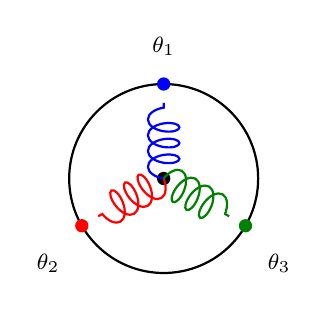
\begin{tikzpicture}[scale=1.2]
    % Ring
    \draw[thick] (0,0) circle (1);

    % Junction center
    \fill (0,0) circle (2pt);

    % Three springs at 120 degrees (equilibrium)
    \foreach \angle/\col in {90/blue, 210/red, 330/green!50!black} {
        \draw[thick,\col,decorate,decoration={coil,aspect=0.5,segment length=2mm,amplitude=2mm}]
            (0,0) -- (\angle:0.8);
        \fill[\col] (\angle:1) circle (2pt);
    }

    % Angles
    \node[above,font=\footnotesize] at (0,1.2) {$\theta_1$};
    \node[below left,font=\footnotesize] at (-1,-0.7) {$\theta_2$};
    \node[below right,font=\footnotesize] at (1,-0.7) {$\theta_3$};
\end{tikzpicture}
\end{center}

\textbf{Interpretation:}
\begin{itemize}[nosep]
    \item Equilibrium: $\theta_1 = \theta_2 = \theta_3 = 120\degree$ (proton)
    \item Excited: angles deviate, springs store extra energy (neutron)
    \item Ring constraint couples all three modes (collective dynamics)
\end{itemize}
\end{tcolorbox}

\subsection{Three-Mode Decomposition}

The junction has three angular degrees of freedom $(\theta_1, \theta_2, \theta_3)$ subject to $\theta_1 + \theta_2 + \theta_3 = 2\pi$. This leaves two independent modes:

\begin{definition}[Mode Decomposition \textup{\tagDef}]
\label{def:modes}
\begin{align}
q &= \text{(collective asymmetry)} = \frac{1}{3}|\hat{e}_1 + \hat{e}_2 + \hat{e}_3| \tag{radial} \\
\perp_1, \perp_2 &= \text{(transverse modes)} \tag{angular}
\end{align}
The collective coordinate $q$ measures overall departure from Steiner; the transverse modes $\perp_{1,2}$ describe shape distortions at fixed $q$.
\end{definition}

\begin{remark}[Effective 1D dynamics \textup{\tagI}]
For slow (adiabatic) relaxation, the transverse modes equilibrate quickly, and the effective dynamics is one-dimensional in $q$. This justifies the 1D WKB treatment in the NJSR paper.
\end{remark}

\subsection{Linearized Oscillation}

Near the metastable neutron configuration $q = q_n$, the dynamics linearizes to:

\begin{equation}
\ddot{q} + 2\gamma \dot{q} + \omega_0^2 (q - q_n) = 0
\label{eq:damped-oscillator}
\end{equation}

where:
\begin{itemize}
    \item $\omega_0$ = natural frequency (junction stiffness) \tagP{}
    \item $\gamma$ = effective damping (energy loss to brane modes) \tagOpen{}
\end{itemize}

\begin{remark}[Not a Standard Model oscillator \textup{\tagI}]
Equation~\eqref{eq:damped-oscillator} is a \textbf{mechanical linearization} around a geometric minimum---not a quantum field theory oscillator. It captures the qualitative behavior: the junction oscillates around its metastable position while losing energy to the brane.
\end{remark}

% ============================================================
%  SECTION 5: PUMPING AND DISSIPATION
% ============================================================
\section{Pumping and Dissipation Pathway}
\label{sec:pumping}

% -----------------------------------------------------------------------------
% CANONICAL PPN (Physical Process Narrative) — CORNERSTONE BOX
% -----------------------------------------------------------------------------
\begin{tcolorbox}[colback=blue!5,colframe=blue!50!black,title=\textbf{Physical Process Narrative (PPN): Bulk $\to$ Brane $\to$ Observer}]
\label{box:ppn}

This section follows the canonical \textbf{PPN framework} for energy transfer in EDC:

\medskip
\begin{enumerate}[nosep,leftmargin=*]
    \item[\textbf{(i)}] \textbf{Bulk cause (5D):} Change in bulk-core configuration $q(t)$ (junction displacement from Steiner) releases geometric energy $\Delta E \approx \Delta m_{np}c^2$.

    \item[\textbf{(ii)}] \textbf{Injection to brane:} This change pumps energy into brane-layer modes $\phi$ at the bulk-facing boundary via $\mathcal{L}_{\mathrm{int}} = g\,q(t)\,\phi(-\delta/2,t)$.

    \item[\textbf{(iii)}] \textbf{Absorption:} The brane accepts the excess energy from the bulk process and stores it as excitations of its degrees of freedom (brane-layer storage).

    \item[\textbf{(iv)}] \textbf{Dissipation/relaxation:} Within the brane-layer, energy redistributes across modes, loses coherence (coarse-graining/decoherence), and flows toward allowed output channels.

    \item[\textbf{(v)}] \textbf{Frozen projection (observer side):} The operator $\mathcal{P}_{\mathrm{frozen}}$ maps brane-layer excitations to observable 3D outputs ($e^- + \bar{\nu}_e + \text{recoil}$), enforcing selection rules.

    \item[\textbf{(vi)}] \textbf{Ledger closure:} Total 5D conservation holds; the brane redirects energy/quantum numbers from bulk channels to observer channels without ``magical disappearance.''
\end{enumerate}

\medskip
\textbf{Epistemic status:} PPN is \tagDef{}/\tagDc{} (narrative bridge); specific mechanisms (dissipation kernel, spectrum, projection details) may be \tagOpen{} where noted.
\end{tcolorbox}

\subsection{Bulk-Core to Brane-Layer Coupling}

As the junction oscillates/relaxes, it couples to modes within the brane layer:

\begin{tcolorbox}[colback=purple!5,colframe=purple!40!black,title=\textbf{Energy Pathway \tagP/\tagOpen}]
\begin{center}
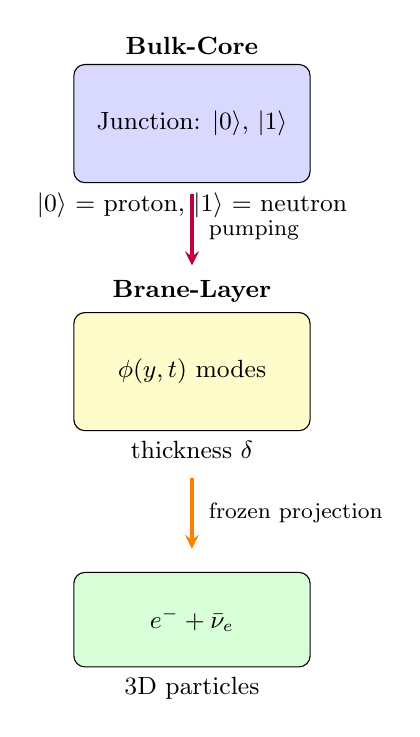
\begin{tikzpicture}[scale=0.9, >=stealth]
    % Bulk core
    \node[draw, rounded corners, fill=blue!15, minimum width=3cm, minimum height=1.5cm] (bulk) at (0,0) {};
    \node[above] at (bulk.north) {\small\textbf{Bulk-Core}};
    \node at (0,0) {\small Junction: $|0\rangle$, $|1\rangle$};
    \node[below,font=\footnotesize] at (bulk.south) {\small $|0\rangle$ = proton, $|1\rangle$ = neutron};

    % Arrow down
    \draw[->,very thick,purple] (0,-1) -- (0,-2);
    \node[right,font=\footnotesize] at (0.1,-1.5) {pumping};

    % Brane layer
    \node[draw, rounded corners, fill=yellow!20, minimum width=3cm, minimum height=1.5cm] (brane) at (0,-3.5) {};
    \node[above] at (brane.north) {\small\textbf{Brane-Layer}};
    \node at (0,-3.5) {\small $\phi(y,t)$ modes};
    \node[below,font=\footnotesize] at (brane.south) {\small thickness $\delta$};

    % Arrow down
    \draw[->,very thick,orange] (0,-5) -- (0,-6);
    \node[right,font=\footnotesize] at (0.1,-5.5) {frozen projection};

    % 3D outputs
    \node[draw, rounded corners, fill=green!15, minimum width=3cm, minimum height=1.2cm] (out) at (0,-7) {};
    \node at (0,-7) {\small $e^- + \bar{\nu}_e$};
    \node[below,font=\footnotesize] at (out.south) {\small 3D particles};
\end{tikzpicture}
\end{center}

\textbf{Mechanism (schematic):}
\begin{enumerate}[nosep]
    \item Neutron junction relaxes: $q_n \to 0$ (toward proton)
    \item Relaxation couples to brane-layer fields: $\mathcal{L}_{\text{int}} \sim g \cdot q(t) \cdot \phi(y=-\delta/2, t)$
    \item Brane modes cascade to observer-facing boundary
    \item Frozen projection selects allowed outputs: $e^- + \bar{\nu}_e + \text{recoil}$
\end{enumerate}
\end{tcolorbox}

\subsection{Coupling Structure}

\begin{postulate}[Bulk-Brane Coupling \textup{\tagP}]
\label{post:coupling}
The junction coordinate $q$ couples linearly to brane-layer modes $\phi$ at the bulk-facing boundary:
\begin{equation}
\mathcal{L}_{\text{int}} = g \, q(t) \, \phi(y = -\delta/2, t)
\label{eq:coupling}
\end{equation}
where $g$ is an effective coupling constant (dimensions and magnitude \tagOpen{}).
\end{postulate}

\noindent\textit{PPN: bulk cause (junction $q$) $\to$ injection (coupling $\mathcal{L}_{\mathrm{int}}$) $\to$ brane absorption $\checkmark$}

\begin{remark}[Coupling derivation \textup{\tagOpen}]
\label{rem:coupling-open}
The coupling Eq.~\eqref{eq:coupling} is postulated based on locality (junction at bulk-facing boundary) and linearity (leading-order expansion). A first-principles derivation from the 5D action remains open.
\end{remark}

\subsection{Conservation Ledger}

\begin{remark}[Energy closure \textup{\tagBL}]
Energy released by junction relaxation ($\Delta E = E(q_n) - E(0) \approx \Delta m_{np} c^2 \approx 1.293$ MeV) is transferred to brane modes and ultimately to 3D particles. Total energy is conserved via Framework v2.0, Remark~4.5.
\end{remark}

\begin{definition}[Energy Partition Ledger \textup{\tagDc}]
\label{def:energy_partition}
The energy released by junction relaxation partitions as:
\begin{equation}
\boxed{\Delta E_{\mathrm{bulk}} = \Delta E_{\mathrm{brane\text{-}layer}} + \Delta E_{\mathrm{residual}}}
\label{eq:energy_partition}
\end{equation}
where:
\begin{itemize}[nosep]
    \item $\Delta E_{\mathrm{bulk}}$: energy lost by bulk-core junction ($\approx \Delta m_{np} c^2$)
    \item $\Delta E_{\mathrm{brane\text{-}layer}}$: energy deposited in brane modes $\phi(y,t)$
    \item $\Delta E_{\mathrm{residual}}$: any energy remaining in bulk (e.g., recoil, radiation)
\end{itemize}
For neutron decay, nearly all energy emerges as 3D particles: $\Delta E_{\mathrm{brane\text{-}layer}} \approx \Delta E_{\mathrm{bulk}}$.
\end{definition}

\noindent\textit{PPN: injection $\to$ absorption (brane storage) $\to$ ledger closure $\checkmark$}

% -----------------------------------------------------------------------------
\subsection{Brane-Layer Dissipation (Effective Damping Model)}
\label{subsec:brane_dissipation}
% -----------------------------------------------------------------------------

The coupling of the junction coordinate $q(t)$ to brane-layer modes induces an effective dissipation. Integrating out the fast brane degrees of freedom yields a damped equation of motion.

\begin{definition}[Effective Damped Equation \textup{\tagP}/\textup{\tagOpen}]
\label{def:damped_eq}
The junction coordinate $q(t)$ satisfies:
\begin{equation}
\boxed{M \ddot{q} + \Gamma \dot{q} + \partial_q V(q) = 0}
\label{eq:damped_motion}
\end{equation}
where:
\begin{itemize}[nosep]
    \item $M$ = effective mass (junction inertia in $q$-space)
    \item $\Gamma$ = effective damping coefficient (brane-layer dissipation)
    \item $V(q)$ = effective potential from junction geometry (Fig.~\ref{fig:potential})
\end{itemize}
\end{definition}

\noindent\textit{PPN: absorption $\to$ dissipation ($\Gamma$ = brane-layer redistribution + decoherence) $\checkmark$}

\begin{remark}[Physical interpretation of $\Gamma$ \textup{\tagP}/\textup{\tagOpen}]
\label{rem:gamma_interpretation}
The coefficient $\Gamma$ encodes the energy transfer rate from the bulk-core junction to brane-layer modes:
\begin{itemize}[nosep]
    \item $\Gamma = 0$: No coupling $\Rightarrow$ undamped oscillation (unphysical)
    \item $\Gamma > 0$: Junction energy drains into brane modes $\Rightarrow$ eventual relaxation
    \item $\Gamma \gg M\omega_0$: Overdamped regime $\Rightarrow$ slow drift toward minimum
\end{itemize}
\textbf{Note:} $\Gamma$ is NOT fitted to the neutron lifetime $\tau_n$ in this companion. Its derivation from thick-brane microphysics remains \tagOpen{}.
\end{remark}

\begin{remark}[Energy partition \textup{\tagDc}/\textup{\tagP}]
From the damped equation~\eqref{eq:damped_motion}, the energy dissipated over time $t$ is:
\begin{equation}
\Delta E_{\mathrm{dissipated}} = \int_0^t \Gamma \dot{q}^2 \, dt' \leq E_{\mathrm{initial}}
\end{equation}
This dissipated energy flows through the brane layer and ultimately emerges as 3D particle kinetic energy via the frozen projection boundary (\S\ref{sec:frozen}).
\end{remark}

\begin{remark}[Connection to WKB treatment \textup{\tagI}/\textup{\tagOpen}]
\label{rem:wkb_bridge}
The NJSR paper computes the neutron lifetime via WKB tunneling through the barrier $V_B$, giving:
\begin{equation}
\tau_n^{-1} = \nu_0 \exp\bigl(-2S/\hbar\bigr) \quad \text{where } S = \int \sqrt{2M V(q)} \, dq
\end{equation}
The damped model here describes the \emph{classical} relaxation pathway. The connection between $\Gamma$ (damping) and $\nu_0$ (attempt frequency) remains an open problem---one expects $\nu_0 \sim \omega_0 \sim \sqrt{\kappa_q/M}$ but the mapping $\Gamma \leftrightarrow \nu_0$ is not yet established.
\end{remark}

% -----------------------------------------------------------------------------
\subsection{Two-Regime Process Model: Charging $\to$ Trigger $\to$ Release}
\label{subsec:two_regime}
% -----------------------------------------------------------------------------

The complete neutron decay process can be understood as passing through two distinct regimes, separated by a trigger event defined by bulk relaxation completion.

\begin{tcolorbox}[colback=green!5,colframe=green!50!black,title=\textbf{Physical Process Narrative: Charging $\to$ Trigger $\to$ Release \tagP}]
\label{box:charging_release}

\textbf{Canonical description:}\\
While the junction relaxes toward the Steiner minimum ($q \to 0$), energy \textbf{pumps} from the bulk-core into the brane-layer, where it is \textbf{stored} as mode excitations (``charging''). When the bulk relaxation enters a regime where pumping becomes negligible compared to release---i.e., the effective description transitions from continuous relaxation to event-like (step)---the brane \textbf{releases} the stored energy budget through frozen projection into allowed 3D outputs.

\medskip
\textbf{Two regimes:}
\begin{enumerate}[nosep,leftmargin=*]
    \item[\textbf{(A)}] \textbf{Charging phase (bulk $\to$ brane):}
    \begin{itemize}[nosep]
        \item Junction relaxation ($q_n \to 0$) drives energy transfer
        \item Coupling: $\mathcal{L}_{\mathrm{int}} = g\,q(t)\,\phi(-\delta/2,t)$
        \item Energy flows as inflow: $J^\nu_{\mathrm{bulk}\to\mathrm{brane}} > 0$
        \item Brane \textbf{absorbs} and \textbf{stores} the energy budget $\mathcal{E}_{\mathrm{brane}}(t)$
    \end{itemize}

    \item[\textbf{(B)}] \textbf{Release phase (brane $\to$ 3D):}
    \begin{itemize}[nosep]
        \item Stored brane-layer energy excites \textbf{brane-layer modes} $\{\phi_k\}$
        \item Modes propagate to observer-facing boundary
        \item Frozen projection $\mathcal{P}_{\mathrm{frozen}}$ maps modes to \textbf{3D particle outputs}
        \item Selection rules filter allowed channels: $e^- + \bar{\nu}_e + \text{recoil}$
    \end{itemize}
\end{enumerate}
\end{tcolorbox}

% =============================================================================
% CANONICAL GLOSSARY BOX: Absorption → Dissipation → Release
% =============================================================================
\begin{tcolorbox}[colback=yellow!5,colframe=orange!60!black,title=\textbf{Canonical Brane-Language for Neutron Decay \tagDef}]
\label{box:canonical_glossary}

The neutron decay process involves \textbf{three conceptually distinct phases}, all part of a single energy-conserving flow:

\medskip
\textbf{(1) Absorption / Charging} (bulk $\to$ brane-layer) \tagDc{}\\
The brane \textbf{receives} energy from the relaxing bulk-core junction. This is not ``creation''---it is \emph{transfer} governed by the coupling $\mathcal{L}_{\mathrm{int}}$.

\smallskip
\emph{Ledger:} $\Delta E_{\mathrm{brane}} = -\Delta E_{\mathrm{bulk}} - E_{\mathrm{other}}$

\medskip
\textbf{(2) Dissipation / Redistribution} (within brane-layer) \tagP{}/\tagOpen{}\\
Internal brane-layer dynamics \textbf{redistribute} the absorbed energy into allowed mode excitations $\{\phi_k\}$. ``Dissipation'' does \textbf{not} mean energy loss---it means transition from coherent pumping channel to spectral mode distribution.

\smallskip
\emph{Mechanism:} Characterized by $\Gamma_{\mathrm{eff}}$ (effective redistribution rate); form \tagOpen{}.

\medskip
\textbf{(3) Release / Emission} (brane-layer $\to$ 3D observer) \tagDc{}/\tagP{}\\
The frozen projection operator $\mathcal{P}_{\mathrm{frozen}}$ \textbf{maps} brane-layer modes to allowed 3D particle outputs. This is \emph{not} ``particle creation from nothing''---it is a boundary projection enforcing selection rules.

\smallskip
\emph{Output:} $\{\phi_k\} \xrightarrow{\mathcal{P}_{\mathrm{frozen}}} \{e^-, \bar{\nu}_e, \mathrm{recoil}, \mathrm{soft}\}_{\mathrm{3D}}$

\medskip
\hrule
\medskip
\textbf{One-liner (citable):}
\begin{quote}
\emph{``Neutron decay in EDC is bulk-core relaxation that charges the brane (absorption), the brane redistributes energy into layer modes (dissipation), and the observer-facing boundary projects those modes into allowed 3D particle outputs (release).''}
\end{quote}
\end{tcolorbox}

% --- Regime-switch interpretation ---
\begin{remark}[Regime-switch interpretation \textup{\tagP}]
\label{rem:regime_switch}
The condition at $t_*$ is \textbf{not} ``$\dot{q} = 0$'' in a literal sense. Instead, $t_*$ marks a \textbf{transition of effective description}: the continuous relaxation of $q(t)$ enters a regime where ongoing pumping is negligible compared to the release channel.

We encode this via a dimensionless \textbf{regime parameter}:
\begin{equation}
\Xi(t) \equiv \frac{\Pi_{\mathrm{pump}}(t)}{\Pi_{\mathrm{release}}(t)} \quad \text{(ratio of transfer/release rates)}
\label{eq:regime_param}
\end{equation}
The trigger condition becomes \tagDef{}/\tagP{}:
\begin{equation}
\boxed{\mathcal{T}_{n\to p}:\quad q(t_*) \approx 0 \quad \land \quad \Xi(t_*) \ll 1}
\label{eq:trigger}
\end{equation}
\textbf{Interpretation:} In this regime, pumping is no longer dominant; the process becomes event-like (step), and the frozen-projection map $\mathcal{P}_{\mathrm{frozen}}$ governs the observable outputs.

\medskip
\noindent\textit{Practical asymptotic condition:} We treat $\Xi \ll 1$ as equivalent to ``pumping power $\Pi_{\mathrm{pump}} \sim \dot{q}\,\partial_q V$ becomes negligible.'' This avoids the question ``how does $\dot{q}$ reach exactly zero in finite time?''
\end{remark}

% --- Charging integral ---
\begin{definition}[Charging Integral \textup{\tagDef}/\textup{\tagOpen}]
\label{def:charging_integral}
The stored brane energy at time $t$ is defined by the integral:
\begin{equation}
\boxed{\mathcal{E}_{\mathrm{brane}}(t) \equiv \int_{t_i}^{t} \Pi_{\mathrm{pump}}(t')\,dt' \quad\text{with}\quad \mathcal{E}_{\mathrm{brane}}(t_*) = \Delta E_{\mathrm{brane}}}
\label{eq:charging_integral}
\end{equation}
where $\Pi_{\mathrm{pump}}(t)$ is the instantaneous power transfer rate (bulk $\to$ brane). The functional form of $\Pi_{\mathrm{pump}}$ depends on $(g, \Gamma, \delta, \ldots)$ and remains \tagOpen{} until derived from brane microphysics.
\end{definition}

% --- Charging ledger with E_other breakdown ---
\begin{definition}[Charging Ledger \textup{\tagDc}]
\label{def:charging_ledger}
During the charging phase, energy conservation requires:
\begin{equation}
\boxed{\Delta E_{\mathrm{brane}} = -\Delta E_{\mathrm{bulk}} - E_{\mathrm{other}}}
\label{eq:charging_ledger}
\end{equation}
where:
\begin{itemize}[nosep]
    \item $\Delta E_{\mathrm{bulk}} = E(q{=}0) - E(q{=}q_n) < 0$ \quad (bulk loses geometric excitation energy)
    \item $\Delta E_{\mathrm{brane}} > 0$ \quad (brane gains stored energy)
\end{itemize}
The residual term $E_{\mathrm{other}}$ decomposes as \tagDc{}/\tagP{}:
\begin{equation}
E_{\mathrm{other}} = E_{\mathrm{recoil}} + E_{\mathrm{soft}} + E_{\mathrm{bulk\,residual}}
\label{eq:e_other}
\end{equation}
\begin{itemize}[nosep]
    \item $E_{\mathrm{recoil}}$: 3D momentum balance (proton recoil) \tagDc{}
    \item $E_{\mathrm{soft}}$: low-energy brane modes, soft photons/phonons \tagP{}
    \item $E_{\mathrm{bulk\,residual}}$: any energy remaining in bulk (if leakage permitted) \tagP{}/\tagOpen{}
\end{itemize}
For neutron decay: $|\Delta E_{\mathrm{bulk}}| \approx \Delta m_{np} c^2 \approx 1.293$ MeV \tagBL{}.
\end{definition}

% --- Energy Bookkeeping Table ---
\begin{table}[htbp]
\centering
\caption{Energy Bookkeeping for Neutron $\beta^-$ Decay \tagDc{}/\tagP{}}
\label{tab:energy_bookkeeping}
\small
\begin{tabular}{@{}lllll@{}}
\toprule
\textbf{Term} & \textbf{Meaning} & \textbf{Tag} & \textbf{Units} & \textbf{Location} \\
\midrule
$\Delta E_{\mathrm{bulk}}$ & Junction relaxation energy & \tagDc{} & MeV & Bulk-core \\
$\Delta E_{\mathrm{brane}}$ & Stored brane energy (charging) & \tagDc{} & MeV & Brane-layer \\
$E_e$ & Electron kinetic + rest mass & \tagBL{} & MeV & 3D output \\
$E_{\bar{\nu}}$ & Antineutrino energy & \tagBL{} & MeV & 3D output \\
$E_{\mathrm{recoil}}$ & Proton recoil & \tagDc{} & keV & 3D output \\
$E_{\mathrm{soft}}$ & Soft photons/phonons & \tagP{} & $\ll$ keV & Brane/3D \\
$E_{\mathrm{bulk\,res.}}$ & Bulk residual (if any) & \tagP{}/\tagOpen{} & — & Bulk \\
\midrule
\multicolumn{5}{@{}l@{}}{\textbf{Conservation check:} $|\Delta E_{\mathrm{bulk}}| = \Delta E_{\mathrm{brane}} + E_{\mathrm{other}}$} \\
\multicolumn{5}{@{}l@{}}{\textbf{Release check:} $\Delta E_{\mathrm{brane}} = E_e + E_{\bar{\nu}} + E_{\mathrm{recoil}} + E_{\mathrm{soft}}$} \\
\midrule
\multicolumn{5}{@{}l@{}}{\textbf{Numerical benchmark} \tagBL{}: $|\Delta E_{\mathrm{bulk}}| \approx 1.293$ MeV (PDG neutron--proton mass difference)} \\
\bottomrule
\end{tabular}
\end{table}

% =============================================================================
% ENERGY-FLOW FIGURE: Bulk → Brane → 3D with ledger closure
% =============================================================================
\begin{figure}[htbp]
\centering
\begin{tikzpicture}[
    node distance=1.8cm and 2.2cm,
    box/.style={rectangle, draw, rounded corners, minimum width=2.8cm, minimum height=0.9cm, align=center, font=\small},
    bulkbox/.style={box, fill=red!10, draw=red!60!black},
    branebox/.style={box, fill=green!10, draw=green!60!black},
    outbox/.style={box, fill=blue!10, draw=blue!60!black},
    arrow/.style={->, >=stealth, thick},
    label/.style={font=\scriptsize, midway, above}
]

% Bulk-core (left)
\node[bulkbox] (bulk) {Bulk excited junction\\$|n\rangle: q > 0$};

% Pumping arrow and label
\node[right=of bulk, branebox] (charge) {Brane energy store\\$\mathcal{E}_{\mathrm{brane}}(t)$};
\draw[arrow, red!70!black] (bulk) -- node[label] {$\Pi_{\mathrm{pump}}$} (charge);

% Brane-layer modes
\node[right=of charge, branebox] (modes) {Layer modes\\$\{\phi_k\}$};
\draw[arrow, green!60!black] (charge) -- node[label] {$\Pi_{\mathrm{release}}$} (modes);

% Frozen projection
\node[right=of modes, outbox] (frozen) {$\mathcal{P}_{\mathrm{frozen}}$};
\draw[arrow, blue!60!black] (modes) -- (frozen);

% 3D outputs
\node[right=of frozen, outbox] (output) {3D outputs\\$e^-, \bar{\nu}_e, \ldots$};
\draw[arrow, blue!60!black] (frozen) -- (output);

% Phase labels below
\node[below=0.3cm of bulk, font=\scriptsize\itshape, red!60!black] {5D Cause};
\node[below=0.3cm of charge, font=\scriptsize\itshape, green!60!black] {Absorption};
\node[below=0.3cm of modes, font=\scriptsize\itshape, green!60!black] {Dissipation};
\node[below=0.3cm of frozen, font=\scriptsize\itshape, blue!60!black] {Projection};
\node[below=0.3cm of output, font=\scriptsize\itshape, blue!60!black] {3D Observation};

% Regime indicator
\node[above=0.6cm of charge, font=\scriptsize] {$\Xi(t) = \Pi_{\mathrm{pump}}/\Pi_{\mathrm{release}}$};
\node[above=1.1cm of modes, font=\scriptsize] {Trigger: $\Xi(t_*) \ll 1$};

% Ledger closure annotation
\draw[dashed, gray] ([yshift=-1.2cm]bulk.south west) -- ([yshift=-1.2cm]output.south east);
\node[below=1.4cm of charge, font=\scriptsize, align=center] {Ledger: $|\Delta E_{\mathrm{bulk}}| = \Delta E_{\mathrm{brane}} + E_{\mathrm{other}}$};

\end{tikzpicture}
\caption{Energy-flow and ledger closure in the neutron $\to$ proton transition. Pumping from bulk-core relaxation charges the brane ($\Pi_{\mathrm{pump}}$); internal redistribution populates layer modes ($\Pi_{\mathrm{release}}$); frozen projection maps modes to allowed 3D outputs. The trigger occurs when $\Xi(t_*) \ll 1$ (pumping negligible). Ledger closure ensures 5D energy conservation.}
\label{fig:energy_flow}
\end{figure}

\begin{remark}[Figure interpretation \textup{\tagDef}]
\label{rem:figure_interpretation}
Figure~\ref{fig:energy_flow} visualizes the canonical narrative:
\begin{itemize}[nosep]
    \item \textbf{Pumping continues while $\Xi \gtrsim 1$}: bulk relaxation dominates.
    \item \textbf{Trigger is regime-switch, not timer}: when $\Xi \ll 1$, release takes over.
    \item \textbf{Release is boundary/projection, not fit}: the frozen operator enforces selection rules.
    \item \textbf{Ledger closes in 5D}: total energy conserved across bulk--brane--3D.
\end{itemize}
\end{remark}

% --- Dimensional definitions for power terms ---
\begin{definition}[Pumping and Release Power \textup{\tagDef}/\textup{\tagOpen}]
\label{def:power_terms}
The power terms appearing in the regime parameter $\Xi(t)$ are defined as:

\medskip
\textbf{(a) Pumping power} (bulk $\to$ brane transfer rate):
\begin{equation}
\boxed{\Pi_{\mathrm{pump}}(t) \equiv -\dot{q}(t) \cdot \partial_q V(q)\big|_{q=q(t)} \quad [\mathrm{units:\ energy/time}]}
\label{eq:pi_pump}
\end{equation}
Physical interpretation: power delivered by the relaxing junction into the coupling interface. When $\dot{q} < 0$ (relaxation toward $q=0$) and $\partial_q V > 0$ (uphill from neutron side), the product is positive.

\medskip
\textbf{(b) Release power} (brane $\to$ 3D emission rate):
\begin{equation}
\boxed{\Pi_{\mathrm{release}}(t) \equiv \Gamma_{\mathrm{eff}} \cdot \mathcal{E}_{\mathrm{brane}}(t) \quad [\mathrm{units:\ energy/time}]}
\label{eq:pi_release}
\end{equation}
where $\Gamma_{\mathrm{eff}}$ is an effective emission rate ($[\mathrm{time}^{-1}]$) characterizing how fast brane-layer modes can transfer into 3D-detectable outputs via frozen projection.

\medskip
\textbf{Note:} Both $\partial_q V$ and $\Gamma_{\mathrm{eff}}$ remain \tagOpen{} until derived from thick-brane microphysics. The definitions above are \textbf{dimensional placeholders} ensuring $\Xi(t) = \Pi_{\mathrm{pump}}/\Pi_{\mathrm{release}}$ is dimensionless.
\end{definition}

% --- Two-step release map ---
\begin{definition}[Two-Step Release Map \textup{\tagDc}/\textup{\tagP}]
\label{def:release_map}
After trigger $\mathcal{T}_{n\to p}$, the stored energy releases in two conceptual steps:
\begin{equation}
\boxed{
\Delta E_{\mathrm{brane}} \;\longrightarrow\; \{\text{brane-layer modes } \phi_k\}
\;\xrightarrow{\mathcal{P}_{\mathrm{frozen}}}\;
\{e^-, \bar{\nu}_e, \text{recoil}, \ldots\}_{\mathrm{3D}}
}
\label{eq:release_map}
\end{equation}
\begin{itemize}[nosep]
    \item \textbf{Step 1} \tagDc{}: Stored energy excites brane-layer modes (ledger transfer)
    \item \textbf{Step 2} \tagP{}/\tagOpen{}: Frozen projection maps modes to 3D particle outputs
\end{itemize}
\textbf{Key point:} Particles are \textbf{not} ``created in the brane''---the brane has modes, and $\mathcal{P}_{\mathrm{frozen}}$ organizes them into quantized 3D outputs satisfying selection rules.
\end{definition}

\begin{remark}[One-line summary \textup{\tagDef}]
\label{rem:oneline_summary}
\begin{quote}
\textit{``The brane absorbs energy from the relaxing junction (Charging) and releases it as particles when bulk relaxation enters the release-dominated regime (Release).''}
\end{quote}
\end{remark}

% -----------------------------------------------------------------------------
% EPISTEMIC GUARDRAIL BOX
% -----------------------------------------------------------------------------
\begin{tcolorbox}[colback=gray!5,colframe=gray!60!black,title=\textbf{Epistemic Guardrail: Observation vs.\ Explanation}]
\label{box:epistemic_guardrail}

\textbf{(1) Baseline observable} \tagBL{}:\\
The neutron lifetime $\tau_n = 878.4 \pm 0.5\,\mathrm{s}$ is an \textbf{empirical fact} measured in 3D. It is \textbf{not} a parameter we choose or fit in this companion.

\medskip
\textbf{$\tau_n$ is not a control knob:} We treat $\tau_n$ as a \textbf{benchmark} \tagBL{}, not as a tuning target. Any mapping $\tau_n \leftrightarrow (\Gamma, g, \delta, \ldots)$ is deferred to \tagOpen{} work.

\medskip
\textbf{(2) Theoretical explanation} \tagP{}/\tagDc{}:\\
The EDC claim is that $\tau_n$ is \textbf{explained} (not tuned) by the bulk-to-brane relaxation mechanism:
\begin{itemize}[nosep]
    \item The bulk junction relaxes toward the Steiner ground state
    \item Energy pumps into the brane layer during relaxation
    \item When the regime parameter $\Xi \ll 1$ (pumping negligible), the brane releases stored energy through frozen projection into allowed 3D outputs
\end{itemize}

\medskip
\textbf{(3) Placeholder parameters} \tagOpen{}:\\
Any effective parameters introduced ($\Gamma$, $g$, $\delta$, $\Pi_{\mathrm{pump}}$, etc.) are \textbf{microphysical placeholders} until derived from the brane model. They are \textbf{not} tuned in this manuscript unless explicitly marked \tagCal{}.

\medskip
\textbf{(4) Trigger as regime boundary} \tagDef{}:\\
The ``trigger'' $\mathcal{T}_{n\to p}$ is a \textbf{regime boundary} ($\Xi \ll 1$), not an arbitrary threshold or timer. It marks where the effective description transitions from continuous relaxation to event-like release.
\end{tcolorbox}

% --- Physical Narration Rule ---
\begin{tcolorbox}[colback=blue!3,colframe=blue!40!black,title=\textbf{Physical Narration Rule (Canonical Standard) \tagDef}]
\label{box:narration_rule}
\textbf{Every key equation must be accompanied by a physical narrative stating:}
\begin{enumerate}[nosep]
    \item \textbf{5D cause:} What changes in the bulk-core configuration?
    \item \textbf{Brane response:} How does the brane layer absorb/redistribute energy?
    \item \textbf{3D observable output:} What do observers detect on the 3D side?
\end{enumerate}
This rule eliminates ``numerology smell'' by ensuring every formula has a mechanistic interpretation.
\end{tcolorbox}

\begin{remark}[What is NOT claimed \textup{\tagDef}]
\label{rem:not_claimed}
This charging/release picture does \textbf{not}:
\begin{itemize}[nosep]
    \item Derive $\tau_n$ from first principles (requires deriving $\Gamma$, $g$, $\Pi_{\mathrm{pump}}$, etc.)
    \item Claim Charging and Release are temporally separated (they may overlap)
    \item Specify the detailed dynamics within the brane layer
    \item Fix a numerical value for $\Xi_{\mathrm{crit}}$ (we use $\Xi \ll 1$ as asymptotic regime)
\end{itemize}
The model provides a \textbf{physical narrative} for where energy goes (bulk $\to$ brane) and how it emerges (brane $\to$ 3D)---not a complete dynamical calculation.
\end{remark}

% ============================================================
%  SECTION 6: FROZEN PROJECTION BOUNDARY
% ============================================================
\section{Frozen Projection Boundary}
\label{sec:frozen}

\subsection{One-Way Valve Mechanism}

\begin{proposition}[Asymmetric Flow \textup{\tagDc}/\textup{\tagP}]
\label{prop:one-way}
The frozen projection boundary acts as a \textbf{one-way valve}:
\begin{itemize}
    \item \textbf{INFLOW} (bulk $\to$ brane): spontaneously allowed
    \item \textbf{OUTFLOW} (brane $\to$ bulk): energetically/kinematically suppressed
\end{itemize}
\end{proposition}

\textbf{Physical interpretation:} The boundary condition at the observer-facing side ``freezes'' high-energy bulk modes, preventing their re-excitation from the 3D side. This is analogous to decoherence: environmental tracing eliminates coherent bulk superpositions.

\subsection{Selection Rules}

The frozen boundary imposes selection rules on which decay products can emerge:

\begin{enumerate}
    \item \textbf{Charge conservation:} $Q_{\text{in}} = Q_{\text{out}}$ (neutron: $0 \to +1 + (-1) + 0$)
    \item \textbf{Lepton number:} $L_e: 0 \to 0 + 1 + (-1) = 0$ (\checkmark)
    \item \textbf{Energy threshold:} $\Delta E > m_e c^2$ required for electron emission
    \item \textbf{Momentum matching:} recoil absorbed by proton
\end{enumerate}

\begin{remark}[V--A structure \textup{\tagBL}]
The $V-A$ (vector minus axial-vector) structure of weak interactions is \textbf{not derived here}---it is input from Standard Model phenomenology. EDC provides the energy release mechanism; the detailed interaction vertex is inherited.
\end{remark}

% -----------------------------------------------------------------------------
\subsection{Formal Frozen Projection Operator}
\label{subsec:frozen_operator}
% -----------------------------------------------------------------------------

We now give a formal definition of the frozen projection, making explicit the mapping from brane-layer modes to observable 3D particles.

\begin{definition}[Brane-Layer Field \textup{\tagDef}]
\label{def:brane_field}
Let $\phi(y, t)$ denote the brane-layer field, where:
\begin{itemize}[nosep]
    \item $y \in [-\delta/2, +\delta/2]$ is the coordinate across the brane thickness $\delta$
    \item $y = -\delta/2$: bulk-facing boundary (where junction couples)
    \item $y = +\delta/2$: observer-facing boundary (where particles emerge)
\end{itemize}
\end{definition}

\begin{definition}[Frozen Projection Operator \textup{\tagDef}/\textup{\tagDc}]
\label{def:frozen_operator}
The \textbf{frozen projection operator} $\mathcal{P}_{\mathrm{frozen}}$ maps brane-layer excitations at the observer-facing boundary to observable 3D particle states:
\begin{equation}
\boxed{\mathcal{P}_{\mathrm{frozen}}: \quad \phi\bigl(y = +\tfrac{\delta}{2}, t\bigr) \;\longmapsto\; \{e^-, e^+, \nu_e, \bar{\nu}_e, \gamma, \ldots\}_{\mathrm{3D}}}
\label{eq:frozen_projection}
\end{equation}
The operator acts as follows:
\begin{enumerate}[nosep]
    \item Identifies modes satisfying the frozen criterion (Def.~\ref{def:frozen_criterion})
    \item Projects these onto mass-shell particle states
    \item Enforces selection rules (charge, lepton number, energy threshold)
\end{enumerate}
\end{definition}

\begin{definition}[Frozen Criterion \textup{\tagDef}/\textup{\tagDc}]
\label{def:frozen_criterion}
A brane-layer mode with characteristic frequency $\omega$ is \textbf{frozen} (appears as a fixed particle rather than a fluctuating field) when:
\begin{equation}
\boxed{\hbar\omega \gg E_{\mathrm{env}}}
\label{eq:frozen_criterion}
\end{equation}
where $E_{\mathrm{env}}$ is the typical environmental energy scale on the 3D side.
\end{definition}

\begin{remark}[Physical interpretation \textup{\tagDc}]
The frozen criterion ensures that high-frequency bulk/brane modes cannot be thermally excited from the 3D side. For neutron decay at room temperature ($E_{\mathrm{env}} \sim k_B T \sim 0.025$ eV), all decay products ($e^-$, $\bar{\nu}_e$ with energies $\sim$ keV--MeV) satisfy $\hbar\omega \gg E_{\mathrm{env}}$ and thus appear as stable particles.
\end{remark}

\begin{remark}[Irreversibility \textup{\tagDc}/\textup{\tagP}]
The frozen projection is effectively \textbf{irreversible}: once energy passes through $\mathcal{P}_{\mathrm{frozen}}$ and materializes as 3D particles, it cannot spontaneously return to bulk-core excitations. This explains why neutron decay is observed but ``inverse beta decay'' ($p + e^- + \bar{\nu}_e \to n$) requires external energy input.
\end{remark}

\noindent\textit{PPN: dissipation $\to$ frozen projection ($\mathcal{P}_{\mathrm{frozen}}$) $\to$ 3D outputs ($e^- + \bar{\nu}_e$) $\to$ ledger closure $\checkmark$}

% ============================================================
%  SECTION 7: BETA DECAY CHANNEL
% ============================================================
\section{Beta$^-$ Channel as Observer-Facing Output}
\label{sec:beta}

\subsection{Decay Process Mapping}

\begin{center}
\begin{tabular}{p{4cm}cp{5cm}}
\toprule
\textbf{5D (Cause)} & & \textbf{3D (Effect)} \\
\midrule
Junction relaxes: $q_n \to 0$ & $\Rightarrow$ & $n \to p$ \\
Energy pumped to brane: $\Delta E \approx 1.293$ MeV & $\Rightarrow$ & Kinetic energy of products \\
Brane modes organize via selection rules & $\Rightarrow$ & $e^- + \bar{\nu}_e$ emission \\
\bottomrule
\end{tabular}
\end{center}

\noindent\textit{PPN complete: bulk cause $\to$ injection $\to$ absorption $\to$ dissipation $\to$ projection $\to$ ledger $\checkmark$}

\subsection{Why Electron and Antineutrino?}

\begin{remark}[Channel selection \textup{\tagDc}/\textup{\tagP}]
The frozen boundary's selection rules (charge, lepton number, energy threshold) determine that:
\begin{itemize}[nosep]
    \item A charge $-1$ lepton must be emitted (to conserve $Q$)
    \item The lightest such lepton is $e^-$ (muon would require $\Delta E > 105$ MeV)
    \item Antineutrino carries lepton number $-1$ (to conserve $L_e$)
\end{itemize}
This is \textbf{not} a derivation of why weak interactions exist, but an explanation of why $\beta^-$ is the allowed channel given the EDC framework.
\end{remark}

\subsection{Suppressed Channels}

\begin{itemize}
    \item $n \to p + \mu^- + \bar{\nu}_\mu$: Forbidden by $m_\mu > \Delta E$
    \item $n \to p + \gamma$: Suppressed (no photon channel in lowest-order weak)
    \item $n \to p + e^- + e^+ + \nu_e + \bar{\nu}_e$: Phase space suppressed
\end{itemize}

% ============================================================
%  SECTION 8: OBSERVABLE BENCHMARKS
% ============================================================
\section{Observable Benchmarks (No Fitting)}
\label{sec:benchmarks}

This section lists observable quantities and their status in the EDC neutron model. \textbf{No parameters are fitted in this companion.}

\begin{center}
\begin{tabular}{lccl}
\toprule
\textbf{Observable} & \textbf{Value} & \textbf{Status} & \textbf{Notes} \\
\midrule
Neutron lifetime $\tau_n$ & $879.4 \pm 0.6$ s & \tagBL{} & PDG 2024 \\
Mass difference $\Delta m_{np}$ & 1.293 MeV & \tagBL{} & CODATA \\
$Q$-value ($n \to p + e + \bar{\nu}$) & 0.782 MeV & \tagBL{} & Kinematic endpoint \\
Proton recoil & $\sim$ keV & \tagBL{} & Small due to mass ratio \\
\midrule
$\Delta m_{np}$ from $\Zsix$ breaking & 1.30 MeV & \tagDc{} & Companion G \\
$q_n \approx 1/3$ & identified & \tagI{} & Half-Steiner \\
Barrier height $V_B$ & $\sim 2.6$ MeV & \tagCal{} & Fitted to $\tau_n$ (NJSR) \\
\bottomrule
\end{tabular}
\end{center}

\begin{remark}[Lifetime is NOT predicted \textup{\tagCal}]
The neutron lifetime $\tau_n \approx 879$ s is reproduced in the NJSR paper via WKB tunneling through a barrier $V_B$. However, $V_B$ is \textbf{calibrated} to match $\tau_n$, not derived from first principles. A first-principles derivation of $V_B$ (or equivalently, the attempt frequency $\Gamma_0$) remains \tagOpen{}.
\end{remark}

% ============================================================
%  SECTION 9: OPEN PROBLEMS
% ============================================================
\section{Open Problems and Research Roadmap}
\label{sec:open}

\subsection{Critical Open Problems}

\begin{enumerate}
    \item \textbf{Derive $V_B$ from 5D action} \tagOpen{}
    \begin{itemize}
        \item Current status: $V_B \approx 2.6$ MeV is calibrated (NJSR paper)
        \item Goal: Show $V_B$ emerges from junction geometry + brane tension
        \item Would upgrade $\tau_n$ from \tagCal{} to \tagDer{}
    \end{itemize}

    \item \textbf{WKB--Damping Bridge} \tagOpen{}
    \begin{itemize}
        \item NJSR paper uses WKB tunneling through $V(q)$
        \item This companion uses damped oscillator + pumping
        \item Goal: Show equivalence in appropriate limits
    \end{itemize}

    \item \textbf{Thick-brane coupling $g$} \tagOpen{}
    \begin{itemize}
        \item Postulated in Eq.~\eqref{eq:coupling}
        \item Need: derive from 5D action or constrain from observables
    \end{itemize}

    \item \textbf{Precise value of $q_n$} \tagI{}/\tagOpen{}
    \begin{itemize}
        \item Currently: $q_n \approx 1/3$ from $\Zsix$ symmetry arguments
        \item Alternative: $q_n \approx 0.31$ from phenomenology
        \item Need: reconcile or derive from first principles
    \end{itemize}
\end{enumerate}

\subsection{Important (For Completeness)}

\begin{itemize}
    \item Derive factor 12 = $\Zsix \times \Ztwo$ connecting 70 MeV and 5.856 MeV scales
    \item Derive $S/\hbar = 60 \approx 12 \ln(1/\alpha) + 1$ (currently \tagI{})
    \item Connect neutrino emission to $\xi$-wave dynamics
\end{itemize}

\subsection{Already Resolved (Documented Elsewhere)}

\begin{center}
\begin{tabular}{lll}
\toprule
\textbf{Problem} & \textbf{Solution} & \textbf{Document} \\
\midrule
Frozen criterion from action & Two routes (instanton + topological) & Framework v2.0 \\
$120\degree$ Steiner angles & Variational derivation & Companion F \\
$\Delta m_{np}$ from geometry & $\Zsix$ symmetry breaking & Companion G \\
Weak channel selection rules & Thick-brane microphysics & Companion H \\
\bottomrule
\end{tabular}
\end{center}

% =============================================================================
%  FALSIFIABILITY AND NON-OVERCLAIM GUARDRAILS
% =============================================================================
\subsection{Falsifiability and Non-Overclaim Guardrails}
\label{subsec:falsifiability}

The charging $\to$ dissipation $\to$ release narrative makes specific structural predictions that could, in principle, falsify or constrain the model:

\begin{enumerate}
    \item \textbf{$E_{\mathrm{other}}$ must have structure} \tagOpen{}\\
    If the ``charging $\to$ release'' picture is correct, the residual energy $E_{\mathrm{other}} = E_{\mathrm{recoil}} + E_{\mathrm{soft}} + E_{\mathrm{bulk\,residual}}$ is \emph{not} arbitrary ``waste''---it has a definite decomposition with physical meaning. If experiments or calculations show $E_{\mathrm{other}}$ lacks this structure (e.g., all energy goes to $e^- + \bar{\nu}$ with no recoil accounting), the ledger picture must be revised.

    \item \textbf{Dissipation must matter if brane-layer is dynamical} \tagP{}/\tagOpen{}\\
    If brane-layer dissipation is physically relevant, then $\Pi_{\mathrm{release}}$ should describe actual mode relaxation dynamics. If it turns out that energy transfer bypasses brane-layer modes entirely (no intermediate $\{\phi_k\}$ step), the dissipation phase is superfluous and the model oversimplifies.

    \item \textbf{Trigger must correlate with pumping cessation} \tagDef{}\\
    The regime parameter $\Xi(t_*) \ll 1$ defines the trigger as ``pumping becomes negligible.'' If observations (or future calculations) show that particle emission occurs \emph{before} pumping becomes negligible---i.e., $\Xi \gtrsim 1$ at emission---then the trigger definition must be revised.

    \item \textbf{Frozen projection must yield allowed outputs only} \tagDc{}/\tagP{}\\
    The $\beta^-$ channel ($e^- + \bar{\nu}_e + p$) is claimed to emerge from frozen projection with selection rules. If it turns out that the selection rules cannot exclude forbidden channels (e.g., $\gamma + p$, $\mu^- + \bar{\nu}_\mu + p$), then either the frozen projection is incomplete or the weak-sector narrative fails.
\end{enumerate}

\begin{tcolorbox}[colback=gray!5,colframe=gray!60!black,title=\textbf{Non-Overclaim Reminder}]
\begin{itemize}[nosep]
    \item $\tau_n = 878.4 \pm 0.5\,\text{s}$ is \tagBL{} (measured), not a control knob.
    \item The mapping $\tau_n \leftrightarrow (\Gamma_{\mathrm{eff}}, g, \delta, V(q))$ remains \tagOpen{}.
    \item This companion provides a \textbf{physical narrative}, not a complete microphysical derivation.
    \item Falsification would require showing the narrative is \emph{inconsistent} with observations or internal logic---not merely incomplete.
\end{itemize}
\end{tcolorbox}

% ============================================================
%  SECTION 10: SUMMARY
% ============================================================
\section{Summary and Epistemic Classification}
\label{sec:summary}

\subsection{Main Results}

\begin{enumerate}
    \item \textbf{Neutron ontology}: Same Y-junction as proton, but excited (displaced from Steiner) \tagP{}

    \item \textbf{Collective coordinate}: $q = |\hat{e}_1 + \hat{e}_2 + \hat{e}_3|/3$ measures asymmetry \tagDef{}

    \item \textbf{Instability}: $q_n > 0$ implies higher energy than proton ($q = 0$) \tagDc{}

    \item \textbf{Relaxation pathway}: Junction $\to$ brane modes $\to$ 3D particles \tagP{}/\tagOpen{}

    \item \textbf{Frozen projection}: Organizes outputs into allowed channels \tagDc{}/\tagP{}
\end{enumerate}

\subsection{Epistemic Classification Table}

\begin{center}
\begin{tabular}{p{4.5cm}cc p{4cm}}
\toprule
\textbf{Claim} & \textbf{Tag} & \textbf{Ref} & \textbf{Notes} \\
\midrule
Baryon = 3-arm junction & \tagP{} & F, Post.~1 & Inherited \\
$120\degree$ Steiner optimum & \tagDer{} & F, Thm.~4.2 & Variational \\
Neutron = excited junction & \tagP{} & Post.~\ref{post:neutron-excited} & This paper \\
Collective coordinate $q$ & \tagDef{} & Def.~\ref{def:collective-q} & Definition \\
Excitation $\Rightarrow$ instability & \tagDc{} & Lem.~\ref{lem:excitation-energy} & From minimum property \\
\midrule
Ring + springs (heuristic) & \tagI{}/\tagP{} & \S\ref{sec:mechanics} & Mechanical analogy \\
Thick-brane pumping & \tagP{}/\tagOpen{} & Post.~\ref{post:coupling} & Mechanism open \\
Frozen projection output & \tagDc{}/\tagP{} & Prop.~\ref{prop:one-way} & From H + Framework v2.0 \\
\midrule
$\tau_n \approx 879$ s & \tagBL{} & PDG & Observable \\
$V_B$ barrier height & \tagCal{} & NJSR paper & Fitted to $\tau_n$ \\
$q_n \approx 1/3$ & \tagI{} & Rem.~\ref{rem:q-neutron} & From $\Zsix$ pattern \\
\bottomrule
\end{tabular}
\end{center}

\subsection{Calibration Boundary}

\textbf{This companion has zero calibrated parameters.}

The neutron lifetime $\tau_n$ enters only as a baseline observable \tagBL{} for consistency checks. The barrier height $V_B$ that determines $\tau_n$ via WKB is calibrated in the NJSR paper (\href{https://doi.org/10.5281/zenodo.18262721}{DOI}), not here. All geometric results ($q$ definition, Steiner instability, relaxation direction) are parameter-free consequences of the junction postulate.

\subsection*{Cornerstone Statement}

\begin{tcolorbox}[colback=blue!5,colframe=blue!40!black,title=\textbf{Neutron Geometry: The Excited Junction Foundation}]
\textbf{Given} the junction postulate (baryons = 3-arm flux-tube networks in 5D, from Companion F):
\begin{enumerate}[nosep]
    \item The neutron is an \textbf{excited} junction state (displaced from Steiner) \tagP{}
    \item Excitation carries geometric energy that drives relaxation \tagDc{}
    \item The collective coordinate $q = |\hat{e}_1 + \hat{e}_2 + \hat{e}_3|/3$ quantifies asymmetry \tagDef{}
    \item Relaxation pumps energy into thick-brane modes \tagP{}/\tagOpen{}
    \item Frozen projection organizes output into $e^- + \bar{\nu}_e$ \tagDc{}/\tagP{}
\end{enumerate}
\textbf{This is the geometric foundation for the neutron in 5D EDC.}

The neutron is not a ``different animal'' from the proton---it is the \textbf{same 5D object} in an excited state, destined to relax toward the Steiner minimum.
\end{tcolorbox}

\vspace{2em}
\hrule
\vspace{1em}
\noindent\textit{Companion N to Paper 3: NJSR Edition}\\
\textit{Draft v0.1: \today}

\end{document}
